\documentclass[1p]{elsarticle_modified}
%\bibliographystyle{elsarticle-num}

%\usepackage[colorlinks]{hyperref}
%\usepackage{abbrmath_seonhwa} %\Abb, \Ascr, \Acal ,\Abf, \Afrak
\usepackage{amsfonts}
\usepackage{amssymb}
\usepackage{amsmath}
\usepackage{amsthm}
\usepackage{scalefnt}
\usepackage{amsbsy}
\usepackage{kotex}
\usepackage{caption}
\usepackage{subfig}
\usepackage{color}
\usepackage{graphicx}
\usepackage{xcolor} %% white, black, red, green, blue, cyan, magenta, yellow
\usepackage{float}
\usepackage{setspace}
\usepackage{hyperref}

\usepackage{tikz}
\usetikzlibrary{arrows}

\usepackage{multirow}
\usepackage{array} % fixed length table
\usepackage{hhline}

%%%%%%%%%%%%%%%%%%%%%
\makeatletter
\renewcommand*\env@matrix[1][\arraystretch]{%
	\edef\arraystretch{#1}%
	\hskip -\arraycolsep
	\let\@ifnextchar\new@ifnextchar
	\array{*\c@MaxMatrixCols c}}
\makeatother %https://tex.stackexchange.com/questions/14071/how-can-i-increase-the-line-spacing-in-a-matrix
%%%%%%%%%%%%%%%

\usepackage[normalem]{ulem}

\newcommand{\msout}[1]{\ifmmode\text{\sout{\ensuremath{#1}}}\else\sout{#1}\fi}
%SOURCE: \msout is \stkout macro in https://tex.stackexchange.com/questions/20609/strikeout-in-math-mode

\newcommand{\cancel}[1]{
	\ifmmode
	{\color{red}\msout{#1}}
	\else
	{\color{red}\sout{#1}}
	\fi
}

\newcommand{\add}[1]{
	{\color{blue}\uwave{#1}}
}

\newcommand{\replace}[2]{
	\ifmmode
	{\color{red}\msout{#1}}{\color{blue}\uwave{#2}}
	\else
	{\color{red}\sout{#1}}{\color{blue}\uwave{#2}}
	\fi
}

\newcommand{\Sol}{\mathcal{S}} %segment
\newcommand{\D}{D} %diagram
\newcommand{\A}{\mathcal{A}} %arc


%%%%%%%%%%%%%%%%%%%%%%%%%%%%%5 test

\def\sl{\operatorname{\textup{SL}}(2,\Cbb)}
\def\psl{\operatorname{\textup{PSL}}(2,\Cbb)}
\def\quan{\mkern 1mu \triangleright \mkern 1mu}

\theoremstyle{definition}
\newtheorem{thm}{Theorem}[section]
\newtheorem{prop}[thm]{Proposition}
\newtheorem{lem}[thm]{Lemma}
\newtheorem{ques}[thm]{Question}
\newtheorem{cor}[thm]{Corollary}
\newtheorem{defn}[thm]{Definition}
\newtheorem{exam}[thm]{Example}
\newtheorem{rmk}[thm]{Remark}
\newtheorem{alg}[thm]{Algorithm}

\newcommand{\I}{\sqrt{-1}}
\begin{document}

%\begin{frontmatter}
%
%\title{Boundary parabolic representations of knots up to 8 crossings}
%
%%% Group authors per affiliation:
%\author{Yunhi Cho} 
%\address{Department of Mathematics, University of Seoul, Seoul, Korea}
%\ead{yhcho@uos.ac.kr}
%
%
%\author{Seonhwa Kim} %\fnref{s_kim}}
%\address{Center for Geometry and Physics, Institute for Basic Science, Pohang, 37673, Korea}
%\ead{ryeona17@ibs.re.kr}
%
%\author{Hyuk Kim}
%\address{Department of Mathematical Sciences, Seoul National University, Seoul 08826, Korea}
%\ead{hyukkim@snu.ac.kr}
%
%\author{Seokbeom Yoon}
%\address{Department of Mathematical Sciences, Seoul National University, Seoul, 08826,  Korea}
%\ead{sbyoon15@snu.ac.kr}
%
%\begin{abstract}
%We find all boundary parabolic representation of knots up to 8 crossings.
%
%\end{abstract}
%\begin{keyword}
%    \MSC[2010] 57M25 
%\end{keyword}
%
%\end{frontmatter}

%\linenumbers
%\tableofcontents
%
\newcommand\colored[1]{\textcolor{white}{\rule[-0.35ex]{0.8em}{1.4ex}}\kern-0.8em\color{red} #1}%
%\newcommand\colored[1]{\textcolor{white}{ #1}\kern-2.17ex	\textcolor{white}{ #1}\kern-1.81ex	\textcolor{white}{ #1}\kern-2.15ex\color{red}#1	}

{\Large $\underline{11a_{19}~(K11a_{19})}$}

\setlength{\tabcolsep}{10pt}
\renewcommand{\arraystretch}{1.6}
\vspace{1cm}\begin{tabular}{m{100pt}>{\centering\arraybackslash}m{274pt}}
\multirow{5}{120pt}{
	\centering
	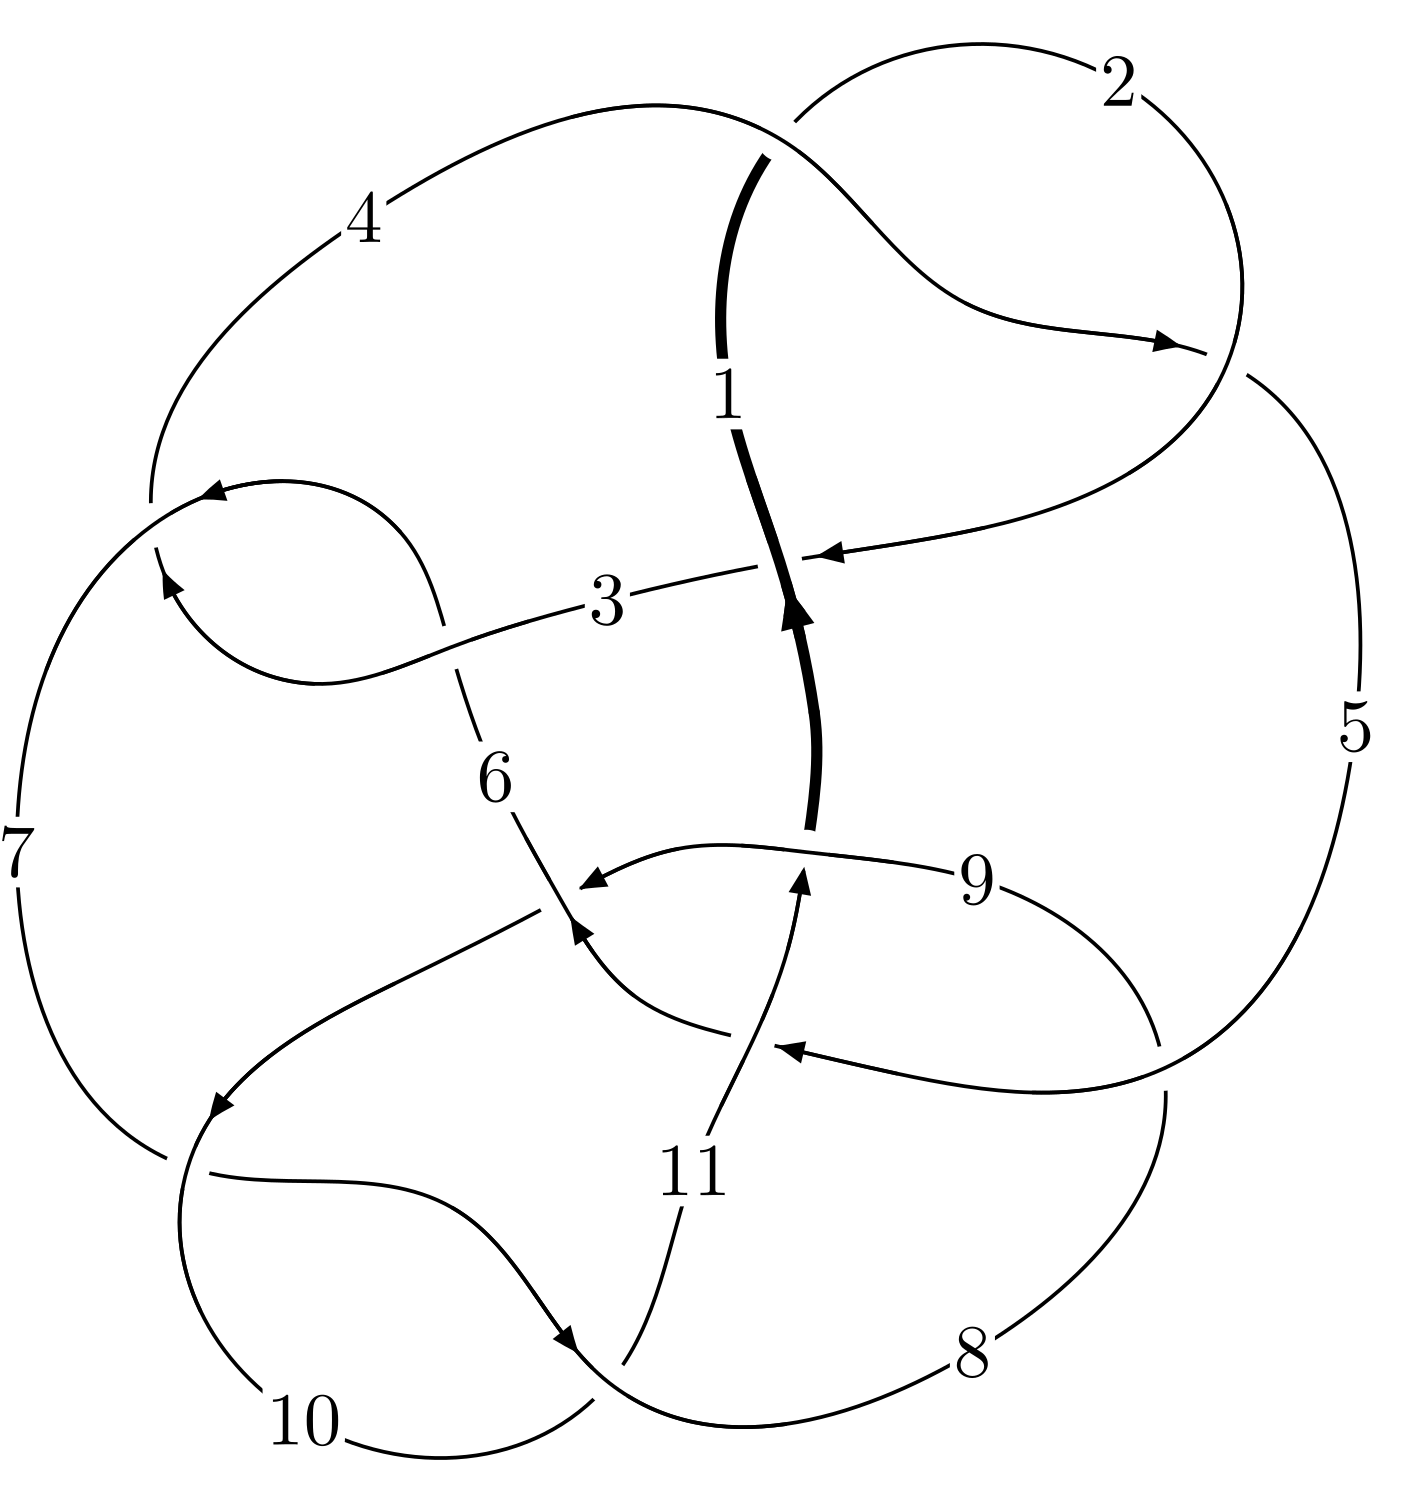
\includegraphics[width=112pt]{../../../GIT/diagram.site/Diagrams/png/268_11a_19.png}\\
\ \ \ A knot diagram\footnotemark}&
\allowdisplaybreaks
\textbf{Linearized knot diagam} \\
\cline{2-2}
 &
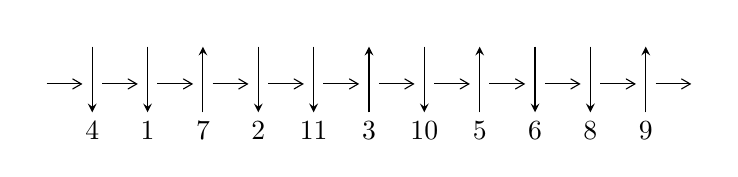
\begin{tikzpicture}[x=20pt, y=17pt]
	% nodes
	\node (C0) at (0, 0) {};
	\node (C1) at (1, 0) {};
	\node (C1U) at (1, +1) {};
	\node (C1D) at (1, -1) {4};

	\node (C2) at (2, 0) {};
	\node (C2U) at (2, +1) {};
	\node (C2D) at (2, -1) {1};

	\node (C3) at (3, 0) {};
	\node (C3U) at (3, +1) {};
	\node (C3D) at (3, -1) {7};

	\node (C4) at (4, 0) {};
	\node (C4U) at (4, +1) {};
	\node (C4D) at (4, -1) {2};

	\node (C5) at (5, 0) {};
	\node (C5U) at (5, +1) {};
	\node (C5D) at (5, -1) {11};

	\node (C6) at (6, 0) {};
	\node (C6U) at (6, +1) {};
	\node (C6D) at (6, -1) {3};

	\node (C7) at (7, 0) {};
	\node (C7U) at (7, +1) {};
	\node (C7D) at (7, -1) {10};

	\node (C8) at (8, 0) {};
	\node (C8U) at (8, +1) {};
	\node (C8D) at (8, -1) {5};

	\node (C9) at (9, 0) {};
	\node (C9U) at (9, +1) {};
	\node (C9D) at (9, -1) {6};

	\node (C10) at (10, 0) {};
	\node (C10U) at (10, +1) {};
	\node (C10D) at (10, -1) {8};

	\node (C11) at (11, 0) {};
	\node (C11U) at (11, +1) {};
	\node (C11D) at (11, -1) {9};
	\node (C12) at (12, 0) {};

	% arrows
	\draw[->,>={angle 60}]
	(C0) edge (C1) (C1) edge (C2) (C2) edge (C3) (C3) edge (C4) (C4) edge (C5) (C5) edge (C6) (C6) edge (C7) (C7) edge (C8) (C8) edge (C9) (C9) edge (C10) (C10) edge (C11) (C11) edge (C12) ;	\draw[->,>=stealth]
	(C1U) edge (C1D) (C2U) edge (C2D) (C3D) edge (C3U) (C4U) edge (C4D) (C5U) edge (C5D) (C6D) edge (C6U) (C7U) edge (C7D) (C8D) edge (C8U) (C9U) edge (C9D) (C10U) edge (C10D) (C11D) edge (C11U) ;
	\end{tikzpicture} \\
\hhline{~~} \\& 
\textbf{Solving Sequence} \\ \cline{2-2} 
 &
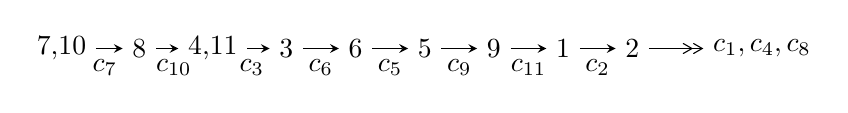
\begin{tikzpicture}[x=25pt, y=7pt]
	% node
	\node (A0) at (-1/8, 0) {7,10};
	\node (A1) at (1, 0) {8};
	\node (A2) at (33/16, 0) {4,11};
	\node (A3) at (25/8, 0) {3};
	\node (A4) at (33/8, 0) {6};
	\node (A5) at (41/8, 0) {5};
	\node (A6) at (49/8, 0) {9};
	\node (A7) at (57/8, 0) {1};
	\node (A8) at (65/8, 0) {2};
	\node (C1) at (1/2, -1) {$c_{7}$};
	\node (C2) at (3/2, -1) {$c_{10}$};
	\node (C3) at (21/8, -1) {$c_{3}$};
	\node (C4) at (29/8, -1) {$c_{6}$};
	\node (C5) at (37/8, -1) {$c_{5}$};
	\node (C6) at (45/8, -1) {$c_{9}$};
	\node (C7) at (53/8, -1) {$c_{11}$};
	\node (C8) at (61/8, -1) {$c_{2}$};
	\node (A9) at (10, 0) {$c_{1},c_{4},c_{8}$};

	% edge
	\draw[->,>=stealth]	
	(A0) edge (A1) (A1) edge (A2) (A2) edge (A3) (A3) edge (A4) (A4) edge (A5) (A5) edge (A6) (A6) edge (A7) (A7) edge (A8) ;
	\draw[->>,>={angle 60}]	
	(A8) edge (A9);
\end{tikzpicture} \\ 

\end{tabular} \\

\footnotetext{
The image of knot diagram is generated by the software ``\textbf{Draw programme}" developed by Andrew Bartholomew(\url{http://www.layer8.co.uk/maths/draw/index.htm\#Running-draw}), where we modified some parts for our purpose(\url{https://github.com/CATsTAILs/LinksPainter}).
}\phantom \\ \newline 
\centering \textbf{Ideals for irreducible components\footnotemark of $X_{\text{par}}$} 
 
\begin{align*}
I^u_{1}&=\langle 
-4.87320\times10^{210} u^{81}-1.20023\times10^{211} u^{80}+\cdots+9.45125\times10^{210} b+3.16425\times10^{211},\\
\phantom{I^u_{1}}&\phantom{= \langle  }-3.92506\times10^{210} u^{81}-1.98955\times10^{211} u^{80}+\cdots+9.45125\times10^{210} a+1.04962\times10^{212},\\
\phantom{I^u_{1}}&\phantom{= \langle  }u^{82}+2 u^{81}+\cdots-14 u+1\rangle \\
I^u_{2}&=\langle 
b,\;u^4+2 u^3- u^2+a-2 u+1,\;u^5+u^4-2 u^3- u^2+u-1\rangle \\
\\
\end{align*}
\raggedright * 2 irreducible components of $\dim_{\mathbb{C}}=0$, with total 87 representations.\\
\footnotetext{All coefficients of polynomials are rational numbers. But the coefficients are sometimes approximated in decimal forms when there is not enough margin.}
\newpage
\renewcommand{\arraystretch}{1}
\centering \section*{I. $I^u_{1}= \langle -4.87\times10^{210} u^{81}-1.20\times10^{211} u^{80}+\cdots+9.45\times10^{210} b+3.16\times10^{211},\;-3.93\times10^{210} u^{81}-1.99\times10^{211} u^{80}+\cdots+9.45\times10^{210} a+1.05\times10^{212},\;u^{82}+2 u^{81}+\cdots-14 u+1 \rangle$}
\flushleft \textbf{(i) Arc colorings}\\
\begin{tabular}{m{7pt} m{180pt} m{7pt} m{180pt} }
\flushright $a_{7}=$&$\begin{pmatrix}1\\0\end{pmatrix}$ \\
\flushright $a_{10}=$&$\begin{pmatrix}0\\u\end{pmatrix}$ \\
\flushright $a_{8}=$&$\begin{pmatrix}1\\u^2\end{pmatrix}$ \\
\flushright $a_{4}=$&$\begin{pmatrix}0.415295 u^{81}+2.10506 u^{80}+\cdots+60.6066 u-11.1056\\0.515615 u^{81}+1.26991 u^{80}+\cdots+34.9413 u-3.34798\end{pmatrix}$ \\
\flushright $a_{11}=$&$\begin{pmatrix}- u\\- u^3+u\end{pmatrix}$ \\
\flushright $a_{3}=$&$\begin{pmatrix}-0.100320 u^{81}+0.835147 u^{80}+\cdots+25.6654 u-7.75762\\0.515615 u^{81}+1.26991 u^{80}+\cdots+34.9413 u-3.34798\end{pmatrix}$ \\
\flushright $a_{6}=$&$\begin{pmatrix}-3.43660 u^{81}-6.69037 u^{80}+\cdots-178.963 u+19.1560\\0.576262 u^{81}+1.37956 u^{80}+\cdots+35.0206 u-4.11670\end{pmatrix}$ \\
\flushright $a_{5}=$&$\begin{pmatrix}-3.52357 u^{81}-6.81623 u^{80}+\cdots-181.274 u+19.5081\\0.650978 u^{81}+1.56146 u^{80}+\cdots+38.0919 u-4.51689\end{pmatrix}$ \\
\flushright $a_{9}=$&$\begin{pmatrix}3.00786 u^{81}+6.93064 u^{80}+\cdots+127.142 u-16.1937\\-0.830021 u^{81}-1.31043 u^{80}+\cdots-9.56980 u+1.53913\end{pmatrix}$ \\
\flushright $a_{1}=$&$\begin{pmatrix}-0.391728 u^{81}-0.569793 u^{80}+\cdots-11.0911 u+0.107632\\0.209315 u^{81}+0.531440 u^{80}+\cdots+14.4741 u-1.32129\end{pmatrix}$ \\
\flushright $a_{2}=$&$\begin{pmatrix}-1.27363 u^{81}-1.06364 u^{80}+\cdots-21.3993 u-3.22549\\0.928834 u^{81}+2.25698 u^{80}+\cdots+59.9874 u-6.00986\end{pmatrix}$\\ \flushright $a_{2}=$&$\begin{pmatrix}-1.27363 u^{81}-1.06364 u^{80}+\cdots-21.3993 u-3.22549\\0.928834 u^{81}+2.25698 u^{80}+\cdots+59.9874 u-6.00986\end{pmatrix}$\\&\end{tabular}
\flushleft \textbf{(ii) Obstruction class $= -1$}\\~\\
\flushleft \textbf{(iii) Cusp Shapes $= -5.57351 u^{81}-11.9801 u^{80}+\cdots-75.2514 u+4.08934$}\\~\\
\newpage\renewcommand{\arraystretch}{1}
\flushleft \textbf{(iv) u-Polynomials at the component}\newline \\
\begin{tabular}{m{50pt}|m{274pt}}
Crossings & \hspace{64pt}u-Polynomials at each crossing \\
\hline $$\begin{aligned}c_{1},c_{4}\end{aligned}$$&$\begin{aligned}
&u^{82}-6 u^{81}+\cdots+8 u-1
\end{aligned}$\\
\hline $$\begin{aligned}c_{2}\end{aligned}$$&$\begin{aligned}
&u^{82}+42 u^{81}+\cdots+32 u+1
\end{aligned}$\\
\hline $$\begin{aligned}c_{3},c_{6}\end{aligned}$$&$\begin{aligned}
&u^{82}- u^{81}+\cdots+160 u+32
\end{aligned}$\\
\hline $$\begin{aligned}c_{5}\end{aligned}$$&$\begin{aligned}
&u^{82}-6 u^{81}+\cdots+2 u-1
\end{aligned}$\\
\hline $$\begin{aligned}c_{7},c_{10}\end{aligned}$$&$\begin{aligned}
&u^{82}-2 u^{81}+\cdots+14 u+1
\end{aligned}$\\
\hline $$\begin{aligned}c_{8}\end{aligned}$$&$\begin{aligned}
&u^{82}-2 u^{81}+\cdots-2362 u-484
\end{aligned}$\\
\hline $$\begin{aligned}c_{9}\end{aligned}$$&$\begin{aligned}
&u^{82}+2 u^{81}+\cdots-20520 u-1647
\end{aligned}$\\
\hline $$\begin{aligned}c_{11}\end{aligned}$$&$\begin{aligned}
&u^{82}+14 u^{81}+\cdots+2 u+1
\end{aligned}$\\
\hline
\end{tabular}\\~\\
\newpage\renewcommand{\arraystretch}{1}
\flushleft \textbf{(v) Riley Polynomials at the component}\newline \\
\begin{tabular}{m{50pt}|m{274pt}}
Crossings & \hspace{64pt}Riley Polynomials at each crossing \\
\hline $$\begin{aligned}c_{1},c_{4}\end{aligned}$$&$\begin{aligned}
&y^{82}-42 y^{81}+\cdots-32 y+1
\end{aligned}$\\
\hline $$\begin{aligned}c_{2}\end{aligned}$$&$\begin{aligned}
&y^{82}+2 y^{81}+\cdots-484 y+1
\end{aligned}$\\
\hline $$\begin{aligned}c_{3},c_{6}\end{aligned}$$&$\begin{aligned}
&y^{82}-33 y^{81}+\cdots-19968 y+1024
\end{aligned}$\\
\hline $$\begin{aligned}c_{5}\end{aligned}$$&$\begin{aligned}
&y^{82}-14 y^{81}+\cdots-6 y+1
\end{aligned}$\\
\hline $$\begin{aligned}c_{7},c_{10}\end{aligned}$$&$\begin{aligned}
&y^{82}-58 y^{81}+\cdots+14 y+1
\end{aligned}$\\
\hline $$\begin{aligned}c_{8}\end{aligned}$$&$\begin{aligned}
&y^{82}+90 y^{81}+\cdots+10862436 y+234256
\end{aligned}$\\
\hline $$\begin{aligned}c_{9}\end{aligned}$$&$\begin{aligned}
&y^{82}+50 y^{81}+\cdots-261288342 y+2712609
\end{aligned}$\\
\hline $$\begin{aligned}c_{11}\end{aligned}$$&$\begin{aligned}
&y^{82}+6 y^{81}+\cdots+14 y+1
\end{aligned}$\\
\hline
\end{tabular}\\~\\
\newpage\flushleft \textbf{(vi) Complex Volumes and Cusp Shapes}
$$\begin{array}{c|c|c}  
\text{Solutions to }I^u_{1}& \I (\text{vol} + \sqrt{-1}CS) & \text{Cusp shape}\\
 \hline 
\begin{aligned}
u &= -0.372669 + 0.922938 I \\
a &= -0.285302 + 0.713657 I \\
b &= \phantom{-}1.210700 - 0.018520 I\end{aligned}
 & \phantom{-}5.22827 - 3.35824 I & \phantom{-0.000000 } 0 \\ \hline\begin{aligned}
u &= -0.372669 - 0.922938 I \\
a &= -0.285302 - 0.713657 I \\
b &= \phantom{-}1.210700 + 0.018520 I\end{aligned}
 & \phantom{-}5.22827 + 3.35824 I & \phantom{-0.000000 } 0 \\ \hline\begin{aligned}
u &= \phantom{-}0.111866 + 0.982814 I \\
a &= \phantom{-}1.122340 + 0.776633 I \\
b &= -0.795431 + 0.455251 I\end{aligned}
 & -2.09067 - 2.95787 I & \phantom{-0.000000 } 0 \\ \hline\begin{aligned}
u &= \phantom{-}0.111866 - 0.982814 I \\
a &= \phantom{-}1.122340 - 0.776633 I \\
b &= -0.795431 - 0.455251 I\end{aligned}
 & -2.09067 + 2.95787 I & \phantom{-0.000000 } 0 \\ \hline\begin{aligned}
u &= -0.948714 + 0.407094 I \\
a &= -0.318376 - 0.441347 I \\
b &= -1.406120 - 0.046993 I\end{aligned}
 & \phantom{-}3.48456 + 2.48996 I & \phantom{-0.000000 } 0 \\ \hline\begin{aligned}
u &= -0.948714 - 0.407094 I \\
a &= -0.318376 + 0.441347 I \\
b &= -1.406120 + 0.046993 I\end{aligned}
 & \phantom{-}3.48456 - 2.48996 I & \phantom{-0.000000 } 0 \\ \hline\begin{aligned}
u &= \phantom{-}1.037470 + 0.112404 I \\
a &= -0.90746 + 3.49927 I \\
b &= -0.959272 + 0.364632 I\end{aligned}
 & -0.006489 - 1.319230 I & \phantom{-0.000000 } 0 \\ \hline\begin{aligned}
u &= \phantom{-}1.037470 - 0.112404 I \\
a &= -0.90746 - 3.49927 I \\
b &= -0.959272 - 0.364632 I\end{aligned}
 & -0.006489 + 1.319230 I & \phantom{-0.000000 } 0 \\ \hline\begin{aligned}
u &= \phantom{-}1.043930 + 0.027951 I \\
a &= \phantom{-}3.12377 + 3.75803 I \\
b &= \phantom{-}0.502899 + 0.690068 I\end{aligned}
 & -3.74856 - 1.03244 I & \phantom{-0.000000 } 0 \\ \hline\begin{aligned}
u &= \phantom{-}1.043930 - 0.027951 I \\
a &= \phantom{-}3.12377 - 3.75803 I \\
b &= \phantom{-}0.502899 - 0.690068 I\end{aligned}
 & -3.74856 + 1.03244 I & \phantom{-0.000000 } 0\\
 \hline 
 \end{array}$$\newpage$$\begin{array}{c|c|c}  
\text{Solutions to }I^u_{1}& \I (\text{vol} + \sqrt{-1}CS) & \text{Cusp shape}\\
 \hline 
\begin{aligned}
u &= \phantom{-}0.924124 + 0.155896 I \\
a &= -1.74666 + 0.78782 I \\
b &= \phantom{-}0.137431 + 0.591455 I\end{aligned}
 & -2.85067 - 0.96287 I & \phantom{-0.000000 } 0 \\ \hline\begin{aligned}
u &= \phantom{-}0.924124 - 0.155896 I \\
a &= -1.74666 - 0.78782 I \\
b &= \phantom{-}0.137431 - 0.591455 I\end{aligned}
 & -2.85067 + 0.96287 I & \phantom{-0.000000 } 0 \\ \hline\begin{aligned}
u &= -0.528336 + 0.760241 I \\
a &= \phantom{-}0.090830 - 1.282120 I \\
b &= -1.209490 - 0.228611 I\end{aligned}
 & \phantom{-}4.80113 + 1.92406 I & \phantom{-0.000000 } 0 \\ \hline\begin{aligned}
u &= -0.528336 - 0.760241 I \\
a &= \phantom{-}0.090830 + 1.282120 I \\
b &= -1.209490 + 0.228611 I\end{aligned}
 & \phantom{-}4.80113 - 1.92406 I & \phantom{-0.000000 } 0 \\ \hline\begin{aligned}
u &= -1.062450 + 0.212626 I \\
a &= -0.49224 - 1.74839 I \\
b &= -1.17978 - 0.78731 I\end{aligned}
 & \phantom{-}0.01560 + 3.91593 I & \phantom{-0.000000 } 0 \\ \hline\begin{aligned}
u &= -1.062450 - 0.212626 I \\
a &= -0.49224 + 1.74839 I \\
b &= -1.17978 + 0.78731 I\end{aligned}
 & \phantom{-}0.01560 - 3.91593 I & \phantom{-0.000000 } 0 \\ \hline\begin{aligned}
u &= \phantom{-}0.055196 + 1.089590 I \\
a &= \phantom{-}0.226034 - 0.928899 I \\
b &= -0.518282 - 0.941047 I\end{aligned}
 & -1.46560 - 5.42569 I & \phantom{-0.000000 } 0 \\ \hline\begin{aligned}
u &= \phantom{-}0.055196 - 1.089590 I \\
a &= \phantom{-}0.226034 + 0.928899 I \\
b &= -0.518282 + 0.941047 I\end{aligned}
 & -1.46560 + 5.42569 I & \phantom{-0.000000 } 0 \\ \hline\begin{aligned}
u &= \phantom{-}1.09577\phantom{ +0.000000I} \\
a &= -5.87610\phantom{ +0.000000I} \\
b &= \phantom{-}0.385176\phantom{ +0.000000I}\end{aligned}
 & -3.80714\phantom{ +0.000000I} & \phantom{-0.000000 } 0 \\ \hline\begin{aligned}
u &= -1.087480 + 0.153969 I \\
a &= -0.10618 - 1.58690 I \\
b &= -0.214732 - 1.243670 I\end{aligned}
 & -2.85407 + 3.43010 I & \phantom{-0.000000 } 0\\
 \hline 
 \end{array}$$\newpage$$\begin{array}{c|c|c}  
\text{Solutions to }I^u_{1}& \I (\text{vol} + \sqrt{-1}CS) & \text{Cusp shape}\\
 \hline 
\begin{aligned}
u &= -1.087480 - 0.153969 I \\
a &= -0.10618 + 1.58690 I \\
b &= -0.214732 + 1.243670 I\end{aligned}
 & -2.85407 - 3.43010 I & \phantom{-0.000000 } 0 \\ \hline\begin{aligned}
u &= -1.099320 + 0.078865 I \\
a &= \phantom{-}0.76703 - 1.64881 I \\
b &= \phantom{-}0.713526 - 1.219340 I\end{aligned}
 & -4.70519 + 2.39134 I & \phantom{-0.000000 } 0 \\ \hline\begin{aligned}
u &= -1.099320 - 0.078865 I \\
a &= \phantom{-}0.76703 + 1.64881 I \\
b &= \phantom{-}0.713526 + 1.219340 I\end{aligned}
 & -4.70519 - 2.39134 I & \phantom{-0.000000 } 0 \\ \hline\begin{aligned}
u &= -1.115110 + 0.022821 I \\
a &= \phantom{-}0.240080 - 1.062120 I \\
b &= \phantom{-}1.243650 - 0.511416 I\end{aligned}
 & -5.52870 + 0.86398 I & \phantom{-0.000000 } 0 \\ \hline\begin{aligned}
u &= -1.115110 - 0.022821 I \\
a &= \phantom{-}0.240080 + 1.062120 I \\
b &= \phantom{-}1.243650 + 0.511416 I\end{aligned}
 & -5.52870 - 0.86398 I & \phantom{-0.000000 } 0 \\ \hline\begin{aligned}
u &= \phantom{-}1.121470 + 0.103386 I \\
a &= \phantom{-}1.55262 - 3.24881 I \\
b &= \phantom{-}1.050130 - 0.595633 I\end{aligned}
 & -2.13971 - 6.01246 I & \phantom{-0.000000 } 0 \\ \hline\begin{aligned}
u &= \phantom{-}1.121470 - 0.103386 I \\
a &= \phantom{-}1.55262 + 3.24881 I \\
b &= \phantom{-}1.050130 + 0.595633 I\end{aligned}
 & -2.13971 + 6.01246 I & \phantom{-0.000000 } 0 \\ \hline\begin{aligned}
u &= \phantom{-}0.817286 + 0.838746 I \\
a &= -0.177044 - 0.087912 I \\
b &= \phantom{-}0.879104 + 0.018096 I\end{aligned}
 & -0.34685 - 2.85468 I & \phantom{-0.000000 } 0 \\ \hline\begin{aligned}
u &= \phantom{-}0.817286 - 0.838746 I \\
a &= -0.177044 + 0.087912 I \\
b &= \phantom{-}0.879104 - 0.018096 I\end{aligned}
 & -0.34685 + 2.85468 I & \phantom{-0.000000 } 0 \\ \hline\begin{aligned}
u &= -0.041190 + 1.176220 I \\
a &= -0.356813 - 0.500680 I \\
b &= \phantom{-}1.110290 - 0.524652 I\end{aligned}
 & \phantom{-}2.93914 - 6.11947 I & \phantom{-0.000000 } 0\\
 \hline 
 \end{array}$$\newpage$$\begin{array}{c|c|c}  
\text{Solutions to }I^u_{1}& \I (\text{vol} + \sqrt{-1}CS) & \text{Cusp shape}\\
 \hline 
\begin{aligned}
u &= -0.041190 - 1.176220 I \\
a &= -0.356813 + 0.500680 I \\
b &= \phantom{-}1.110290 + 0.524652 I\end{aligned}
 & \phantom{-}2.93914 + 6.11947 I & \phantom{-0.000000 } 0 \\ \hline\begin{aligned}
u &= \phantom{-}0.783636 + 0.165518 I \\
a &= \phantom{-}0.38779 + 2.04319 I \\
b &= -0.959378 - 0.173898 I\end{aligned}
 & \phantom{-}0.603497 + 0.216471 I & -3.00000 - 5.07001 I \\ \hline\begin{aligned}
u &= \phantom{-}0.783636 - 0.165518 I \\
a &= \phantom{-}0.38779 - 2.04319 I \\
b &= -0.959378 + 0.173898 I\end{aligned}
 & \phantom{-}0.603497 - 0.216471 I & -3.00000 + 5.07001 I \\ \hline\begin{aligned}
u &= -1.085630 + 0.509853 I \\
a &= \phantom{-}0.180279 + 0.797287 I \\
b &= \phantom{-}1.382850 + 0.228355 I\end{aligned}
 & \phantom{-}2.97750 + 8.50086 I & \phantom{-0.000000 } 0 \\ \hline\begin{aligned}
u &= -1.085630 - 0.509853 I \\
a &= \phantom{-}0.180279 - 0.797287 I \\
b &= \phantom{-}1.382850 - 0.228355 I\end{aligned}
 & \phantom{-}2.97750 - 8.50086 I & \phantom{-0.000000 } 0 \\ \hline\begin{aligned}
u &= -1.190570 + 0.263500 I \\
a &= \phantom{-}0.40339 + 1.85670 I \\
b &= \phantom{-}1.16152 + 0.83000 I\end{aligned}
 & -3.13741 + 9.59200 I & \phantom{-0.000000 } 0 \\ \hline\begin{aligned}
u &= -1.190570 - 0.263500 I \\
a &= \phantom{-}0.40339 - 1.85670 I \\
b &= \phantom{-}1.16152 - 0.83000 I\end{aligned}
 & -3.13741 - 9.59200 I & \phantom{-0.000000 } 0 \\ \hline\begin{aligned}
u &= \phantom{-}0.516137 + 1.108300 I \\
a &= -0.114506 - 0.399456 I \\
b &= -0.916579 - 0.485003 I\end{aligned}
 & -1.65757 + 0.93442 I & \phantom{-0.000000 } 0 \\ \hline\begin{aligned}
u &= \phantom{-}0.516137 - 1.108300 I \\
a &= -0.114506 + 0.399456 I \\
b &= -0.916579 + 0.485003 I\end{aligned}
 & -1.65757 - 0.93442 I & \phantom{-0.000000 } 0 \\ \hline\begin{aligned}
u &= -0.014957 + 0.768895 I \\
a &= -0.717422 + 0.722948 I \\
b &= \phantom{-}0.134543 + 0.766173 I\end{aligned}
 & \phantom{-}0.28541 - 1.54658 I & -0.57343 + 2.06881 I\\
 \hline 
 \end{array}$$\newpage$$\begin{array}{c|c|c}  
\text{Solutions to }I^u_{1}& \I (\text{vol} + \sqrt{-1}CS) & \text{Cusp shape}\\
 \hline 
\begin{aligned}
u &= -0.014957 - 0.768895 I \\
a &= -0.717422 - 0.722948 I \\
b &= \phantom{-}0.134543 - 0.766173 I\end{aligned}
 & \phantom{-}0.28541 + 1.54658 I & -0.57343 - 2.06881 I \\ \hline\begin{aligned}
u &= \phantom{-}0.025777 + 1.279070 I \\
a &= \phantom{-}0.180112 + 0.766794 I \\
b &= -1.131140 + 0.685484 I\end{aligned}
 & \phantom{-}0.45408 - 11.38860 I & \phantom{-0.000000 } 0 \\ \hline\begin{aligned}
u &= \phantom{-}0.025777 - 1.279070 I \\
a &= \phantom{-}0.180112 - 0.766794 I \\
b &= -1.131140 - 0.685484 I\end{aligned}
 & \phantom{-}0.45408 + 11.38860 I & \phantom{-0.000000 } 0 \\ \hline\begin{aligned}
u &= \phantom{-}0.586949 + 0.306956 I \\
a &= -0.394714 - 1.242930 I \\
b &= \phantom{-}1.013700 + 0.500772 I\end{aligned}
 & -0.96667 + 4.63901 I & -3.87963 - 8.57640 I \\ \hline\begin{aligned}
u &= \phantom{-}0.586949 - 0.306956 I \\
a &= -0.394714 + 1.242930 I \\
b &= \phantom{-}1.013700 - 0.500772 I\end{aligned}
 & -0.96667 - 4.63901 I & -3.87963 + 8.57640 I \\ \hline\begin{aligned}
u &= \phantom{-}1.34181\phantom{ +0.000000I} \\
a &= \phantom{-}0.104308\phantom{ +0.000000I} \\
b &= \phantom{-}0.435201\phantom{ +0.000000I}\end{aligned}
 & -2.55123\phantom{ +0.000000I} & \phantom{-0.000000 } 0 \\ \hline\begin{aligned}
u &= -1.294620 + 0.433035 I \\
a &= \phantom{-}0.629514 - 1.164780 I \\
b &= \phantom{-}0.399119 - 1.045250 I\end{aligned}
 & -3.71598 + 6.06156 I & \phantom{-0.000000 } 0 \\ \hline\begin{aligned}
u &= -1.294620 - 0.433035 I \\
a &= \phantom{-}0.629514 + 1.164780 I \\
b &= \phantom{-}0.399119 + 1.045250 I\end{aligned}
 & -3.71598 - 6.06156 I & \phantom{-0.000000 } 0 \\ \hline\begin{aligned}
u &= -1.42187 + 0.12543 I \\
a &= \phantom{-}0.601248 + 0.581607 I \\
b &= \phantom{-}0.535579 + 0.443898 I\end{aligned}
 & -7.77694 + 4.95365 I & \phantom{-0.000000 } 0 \\ \hline\begin{aligned}
u &= -1.42187 - 0.12543 I \\
a &= \phantom{-}0.601248 - 0.581607 I \\
b &= \phantom{-}0.535579 - 0.443898 I\end{aligned}
 & -7.77694 - 4.95365 I & \phantom{-0.000000 } 0\\
 \hline 
 \end{array}$$\newpage$$\begin{array}{c|c|c}  
\text{Solutions to }I^u_{1}& \I (\text{vol} + \sqrt{-1}CS) & \text{Cusp shape}\\
 \hline 
\begin{aligned}
u &= -1.34855 + 0.46968 I \\
a &= \phantom{-}0.39620 - 1.58221 I \\
b &= -1.033970 - 0.543976 I\end{aligned}
 & -6.58899 + 8.11200 I & \phantom{-0.000000 } 0 \\ \hline\begin{aligned}
u &= -1.34855 - 0.46968 I \\
a &= \phantom{-}0.39620 + 1.58221 I \\
b &= -1.033970 + 0.543976 I\end{aligned}
 & -6.58899 - 8.11200 I & \phantom{-0.000000 } 0 \\ \hline\begin{aligned}
u &= -1.36225 + 0.50910 I \\
a &= -0.87526 + 1.16446 I \\
b &= -0.617126 + 1.091420 I\end{aligned}
 & -5.89382 + 11.02700 I & \phantom{-0.000000 } 0 \\ \hline\begin{aligned}
u &= -1.36225 - 0.50910 I \\
a &= -0.87526 - 1.16446 I \\
b &= -0.617126 - 1.091420 I\end{aligned}
 & -5.89382 - 11.02700 I & \phantom{-0.000000 } 0 \\ \hline\begin{aligned}
u &= -1.36047 + 0.56106 I \\
a &= -0.02227 + 1.66535 I \\
b &= \phantom{-}1.189870 + 0.667621 I\end{aligned}
 & -1.22744 + 12.16920 I & \phantom{-0.000000 } 0 \\ \hline\begin{aligned}
u &= -1.36047 - 0.56106 I \\
a &= -0.02227 - 1.66535 I \\
b &= \phantom{-}1.189870 - 0.667621 I\end{aligned}
 & -1.22744 - 12.16920 I & \phantom{-0.000000 } 0 \\ \hline\begin{aligned}
u &= -1.46239 + 0.32296 I \\
a &= -0.756015 + 0.523946 I \\
b &= -0.596900 + 0.506514 I\end{aligned}
 & -8.00907 + 3.75643 I & \phantom{-0.000000 } 0 \\ \hline\begin{aligned}
u &= -1.46239 - 0.32296 I \\
a &= -0.756015 - 0.523946 I \\
b &= -0.596900 - 0.506514 I\end{aligned}
 & -8.00907 - 3.75643 I & \phantom{-0.000000 } 0 \\ \hline\begin{aligned}
u &= \phantom{-}1.31960 + 0.71550 I \\
a &= -0.208693 - 1.217520 I \\
b &= \phantom{-}0.940672 - 0.500766 I\end{aligned}
 & -1.85423 - 3.78257 I & \phantom{-0.000000 } 0 \\ \hline\begin{aligned}
u &= \phantom{-}1.31960 - 0.71550 I \\
a &= -0.208693 + 1.217520 I \\
b &= \phantom{-}0.940672 + 0.500766 I\end{aligned}
 & -1.85423 + 3.78257 I & \phantom{-0.000000 } 0\\
 \hline 
 \end{array}$$\newpage$$\begin{array}{c|c|c}  
\text{Solutions to }I^u_{1}& \I (\text{vol} + \sqrt{-1}CS) & \text{Cusp shape}\\
 \hline 
\begin{aligned}
u &= \phantom{-}1.43309 + 0.47733 I \\
a &= \phantom{-}0.54768 + 1.85069 I \\
b &= -0.676418 + 0.654214 I\end{aligned}
 & -5.91812 - 0.62603 I & \phantom{-0.000000 } 0 \\ \hline\begin{aligned}
u &= \phantom{-}1.43309 - 0.47733 I \\
a &= \phantom{-}0.54768 - 1.85069 I \\
b &= -0.676418 - 0.654214 I\end{aligned}
 & -5.91812 + 0.62603 I & \phantom{-0.000000 } 0 \\ \hline\begin{aligned}
u &= \phantom{-}1.39410 + 0.58186 I \\
a &= -0.362073 - 1.189890 I \\
b &= -0.603714 - 0.799274 I\end{aligned}
 & -5.73183 - 3.04738 I & \phantom{-0.000000 } 0 \\ \hline\begin{aligned}
u &= \phantom{-}1.39410 - 0.58186 I \\
a &= -0.362073 + 1.189890 I \\
b &= -0.603714 + 0.799274 I\end{aligned}
 & -5.73183 + 3.04738 I & \phantom{-0.000000 } 0 \\ \hline\begin{aligned}
u &= \phantom{-}1.49404 + 0.24932 I \\
a &= \phantom{-}0.416319 + 0.504070 I \\
b &= \phantom{-}0.717839 + 0.375621 I\end{aligned}
 & -2.65606 + 0.12519 I & \phantom{-0.000000 } 0 \\ \hline\begin{aligned}
u &= \phantom{-}1.49404 - 0.24932 I \\
a &= \phantom{-}0.416319 - 0.504070 I \\
b &= \phantom{-}0.717839 - 0.375621 I\end{aligned}
 & -2.65606 - 0.12519 I & \phantom{-0.000000 } 0 \\ \hline\begin{aligned}
u &= -1.41333 + 0.57602 I \\
a &= -0.03235 - 1.85061 I \\
b &= -1.169980 - 0.781904 I\end{aligned}
 & -4.0922 + 17.7863 I & \phantom{-0.000000 } 0 \\ \hline\begin{aligned}
u &= -1.41333 - 0.57602 I \\
a &= -0.03235 + 1.85061 I \\
b &= -1.169980 + 0.781904 I\end{aligned}
 & -4.0922 - 17.7863 I & \phantom{-0.000000 } 0 \\ \hline\begin{aligned}
u &= \phantom{-}0.017201 + 0.444698 I \\
a &= -0.421573 + 0.688439 I \\
b &= \phantom{-}1.140810 - 0.618738 I\end{aligned}
 & \phantom{-}0.34729 - 6.79546 I & -2.04718 + 3.52041 I \\ \hline\begin{aligned}
u &= \phantom{-}0.017201 - 0.444698 I \\
a &= -0.421573 - 0.688439 I \\
b &= \phantom{-}1.140810 + 0.618738 I\end{aligned}
 & \phantom{-}0.34729 + 6.79546 I & -2.04718 - 3.52041 I\\
 \hline 
 \end{array}$$\newpage$$\begin{array}{c|c|c}  
\text{Solutions to }I^u_{1}& \I (\text{vol} + \sqrt{-1}CS) & \text{Cusp shape}\\
 \hline 
\begin{aligned}
u &= \phantom{-}0.047106 + 0.410466 I \\
a &= -1.47054 - 0.16933 I \\
b &= -0.217093 + 0.544112 I\end{aligned}
 & \phantom{-}0.041508 - 1.376630 I & \phantom{-}0.16544 + 4.98668 I \\ \hline\begin{aligned}
u &= \phantom{-}0.047106 - 0.410466 I \\
a &= -1.47054 + 0.16933 I \\
b &= -0.217093 - 0.544112 I\end{aligned}
 & \phantom{-}0.041508 + 1.376630 I & \phantom{-}0.16544 - 4.98668 I \\ \hline\begin{aligned}
u &= \phantom{-}1.46595 + 0.77759 I \\
a &= -0.08409 + 1.44082 I \\
b &= -1.043820 + 0.658784 I\end{aligned}
 & -4.37377 - 8.54127 I & \phantom{-0.000000 } 0 \\ \hline\begin{aligned}
u &= \phantom{-}1.46595 - 0.77759 I \\
a &= -0.08409 - 1.44082 I \\
b &= -1.043820 - 0.658784 I\end{aligned}
 & -4.37377 + 8.54127 I & \phantom{-0.000000 } 0 \\ \hline\begin{aligned}
u &= -0.116621 + 0.310795 I \\
a &= -0.295025 - 1.350840 I \\
b &= -1.130240 + 0.389337 I\end{aligned}
 & \phantom{-}2.44851 - 1.57419 I & \phantom{-}1.58009 - 0.44639 I \\ \hline\begin{aligned}
u &= -0.116621 - 0.310795 I \\
a &= -0.295025 + 1.350840 I \\
b &= -1.130240 - 0.389337 I\end{aligned}
 & \phantom{-}2.44851 + 1.57419 I & \phantom{-}1.58009 + 0.44639 I \\ \hline\begin{aligned}
u &= \phantom{-}1.67621 + 0.41894 I \\
a &= -0.801743 - 0.790902 I \\
b &= -0.973653 - 0.605011 I\end{aligned}
 & -5.00012 + 4.29669 I & \phantom{-0.000000 } 0 \\ \hline\begin{aligned}
u &= \phantom{-}1.67621 - 0.41894 I \\
a &= -0.801743 + 0.790902 I \\
b &= -0.973653 + 0.605011 I\end{aligned}
 & -5.00012 - 4.29669 I & \phantom{-0.000000 } 0 \\ \hline\begin{aligned}
u &= \phantom{-}0.182502 + 0.012960 I \\
a &= -5.67324 + 0.60050 I \\
b &= \phantom{-}0.570425 + 0.460109 I\end{aligned}
 & -2.36954 - 0.63816 I & -5.46759 - 1.52326 I \\ \hline\begin{aligned}
u &= \phantom{-}0.182502 - 0.012960 I \\
a &= -5.67324 - 0.60050 I \\
b &= \phantom{-}0.570425 - 0.460109 I\end{aligned}
 & -2.36954 + 0.63816 I & -5.46759 + 1.52326 I\\
 \hline 
 \end{array}$$\newpage$$\begin{array}{c|c|c}  
\text{Solutions to }I^u_{1}& \I (\text{vol} + \sqrt{-1}CS) & \text{Cusp shape}\\
 \hline 
\begin{aligned}
u &= \phantom{-}0.054094 + 0.154978 I \\
a &= -4.35975 - 0.04873 I \\
b &= \phantom{-}0.408288 + 0.821403 I\end{aligned}
 & -1.87549 - 1.38403 I & -4.93593 + 0.98614 I \\ \hline\begin{aligned}
u &= \phantom{-}0.054094 - 0.154978 I \\
a &= -4.35975 + 0.04873 I \\
b &= \phantom{-}0.408288 - 0.821403 I\end{aligned}
 & -1.87549 + 1.38403 I & -4.93593 - 0.98614 I\\
 \hline 
 \end{array}$$\newpage\newpage\renewcommand{\arraystretch}{1}
\centering \section*{II. $I^u_{2}= \langle b,\;u^4+2 u^3- u^2+a-2 u+1,\;u^5+u^4-2 u^3- u^2+u-1 \rangle$}
\flushleft \textbf{(i) Arc colorings}\\
\begin{tabular}{m{7pt} m{180pt} m{7pt} m{180pt} }
\flushright $a_{7}=$&$\begin{pmatrix}1\\0\end{pmatrix}$ \\
\flushright $a_{10}=$&$\begin{pmatrix}0\\u\end{pmatrix}$ \\
\flushright $a_{8}=$&$\begin{pmatrix}1\\u^2\end{pmatrix}$ \\
\flushright $a_{4}=$&$\begin{pmatrix}- u^4-2 u^3+u^2+2 u-1\\0\end{pmatrix}$ \\
\flushright $a_{11}=$&$\begin{pmatrix}- u\\- u^3+u\end{pmatrix}$ \\
\flushright $a_{3}=$&$\begin{pmatrix}- u^4-2 u^3+u^2+2 u-1\\0\end{pmatrix}$ \\
\flushright $a_{6}=$&$\begin{pmatrix}1\\0\end{pmatrix}$ \\
\flushright $a_{5}=$&$\begin{pmatrix}- u^4+u^2+1\\- u^4+u^3+u^2-2 u+1\end{pmatrix}$ \\
\flushright $a_{9}=$&$\begin{pmatrix}u\\u\end{pmatrix}$ \\
\flushright $a_{1}=$&$\begin{pmatrix}u^4- u^2-1\\u^4- u^3- u^2+2 u-1\end{pmatrix}$ \\
\flushright $a_{2}=$&$\begin{pmatrix}-2 u^3+2 u-2\\u^4- u^3- u^2+2 u-1\end{pmatrix}$\\ \flushright $a_{2}=$&$\begin{pmatrix}-2 u^3+2 u-2\\u^4- u^3- u^2+2 u-1\end{pmatrix}$\\&\end{tabular}
\flushleft \textbf{(ii) Obstruction class $= 1$}\\~\\
\flushleft \textbf{(iii) Cusp Shapes $= -3 u^4-7 u^3+2 u^2+6 u-7$}\\~\\
\newpage\renewcommand{\arraystretch}{1}
\flushleft \textbf{(iv) u-Polynomials at the component}\newline \\
\begin{tabular}{m{50pt}|m{274pt}}
Crossings & \hspace{64pt}u-Polynomials at each crossing \\
\hline $$\begin{aligned}c_{1}\end{aligned}$$&$\begin{aligned}
&(u-1)^5
\end{aligned}$\\
\hline $$\begin{aligned}c_{2},c_{4}\end{aligned}$$&$\begin{aligned}
&(u+1)^5
\end{aligned}$\\
\hline $$\begin{aligned}c_{3},c_{6}\end{aligned}$$&$\begin{aligned}
&u^5
\end{aligned}$\\
\hline $$\begin{aligned}c_{5}\end{aligned}$$&$\begin{aligned}
&u^5-3 u^4+4 u^3- u^2- u+1
\end{aligned}$\\
\hline $$\begin{aligned}c_{7}\end{aligned}$$&$\begin{aligned}
&u^5+u^4-2 u^3- u^2+u-1
\end{aligned}$\\
\hline $$\begin{aligned}c_{8},c_{11}\end{aligned}$$&$\begin{aligned}
&u^5+u^4+2 u^3+u^2+u+1
\end{aligned}$\\
\hline $$\begin{aligned}c_{9},c_{10}\end{aligned}$$&$\begin{aligned}
&u^5- u^4-2 u^3+u^2+u+1
\end{aligned}$\\
\hline
\end{tabular}\\~\\
\newpage\renewcommand{\arraystretch}{1}
\flushleft \textbf{(v) Riley Polynomials at the component}\newline \\
\begin{tabular}{m{50pt}|m{274pt}}
Crossings & \hspace{64pt}Riley Polynomials at each crossing \\
\hline $$\begin{aligned}c_{1},c_{2},c_{4}\end{aligned}$$&$\begin{aligned}
&(y-1)^5
\end{aligned}$\\
\hline $$\begin{aligned}c_{3},c_{6}\end{aligned}$$&$\begin{aligned}
&y^5
\end{aligned}$\\
\hline $$\begin{aligned}c_{5}\end{aligned}$$&$\begin{aligned}
&y^5- y^4+8 y^3-3 y^2+3 y-1
\end{aligned}$\\
\hline $$\begin{aligned}c_{7},c_{9},c_{10}\end{aligned}$$&$\begin{aligned}
&y^5-5 y^4+8 y^3-3 y^2- y-1
\end{aligned}$\\
\hline $$\begin{aligned}c_{8},c_{11}\end{aligned}$$&$\begin{aligned}
&y^5+3 y^4+4 y^3+y^2- y-1
\end{aligned}$\\
\hline
\end{tabular}\\~\\
\newpage\flushleft \textbf{(vi) Complex Volumes and Cusp Shapes}
$$\begin{array}{c|c|c}  
\text{Solutions to }I^u_{2}& \I (\text{vol} + \sqrt{-1}CS) & \text{Cusp shape}\\
 \hline 
\begin{aligned}
u &= \phantom{-}1.21774\phantom{ +0.000000I} \\
a &= -2.89210\phantom{ +0.000000I} \\
b &= \phantom{-0.000000 } 0\end{aligned}
 & -4.04602\phantom{ +0.000000I} & -15.9650\phantom{ +0.000000I} \\ \hline\begin{aligned}
u &= \phantom{-}0.309916 + 0.549911 I \\
a &= -0.01014 + 1.59703 I \\
b &= \phantom{-0.000000 } 0\end{aligned}
 & -1.97403 - 1.53058 I & -3.57269 + 4.45807 I \\ \hline\begin{aligned}
u &= \phantom{-}0.309916 - 0.549911 I \\
a &= -0.01014 - 1.59703 I \\
b &= \phantom{-0.000000 } 0\end{aligned}
 & -1.97403 + 1.53058 I & -3.57269 - 4.45807 I \\ \hline\begin{aligned}
u &= -1.41878 + 0.21917 I \\
a &= -0.043806 - 0.365575 I \\
b &= \phantom{-0.000000 } 0\end{aligned}
 & -7.51750 + 4.40083 I & -3.44484 - 1.78781 I \\ \hline\begin{aligned}
u &= -1.41878 - 0.21917 I \\
a &= -0.043806 + 0.365575 I \\
b &= \phantom{-0.000000 } 0\end{aligned}
 & -7.51750 - 4.40083 I & -3.44484 + 1.78781 I\\
 \hline 
 \end{array}$$\newpage
\newpage\renewcommand{\arraystretch}{1}
\centering \section*{ III. u-Polynomials}
\begin{tabular}{m{50pt}|m{274pt}}
Crossings & \hspace{64pt}u-Polynomials at each crossing \\
\hline $$\begin{aligned}c_{1}\end{aligned}$$&$\begin{aligned}
&((u-1)^5)(u^{82}-6 u^{81}+\cdots+8 u-1)
\end{aligned}$\\
\hline $$\begin{aligned}c_{2}\end{aligned}$$&$\begin{aligned}
&((u+1)^5)(u^{82}+42 u^{81}+\cdots+32 u+1)
\end{aligned}$\\
\hline $$\begin{aligned}c_{3},c_{6}\end{aligned}$$&$\begin{aligned}
&u^5(u^{82}- u^{81}+\cdots+160 u+32)
\end{aligned}$\\
\hline $$\begin{aligned}c_{4}\end{aligned}$$&$\begin{aligned}
&((u+1)^5)(u^{82}-6 u^{81}+\cdots+8 u-1)
\end{aligned}$\\
\hline $$\begin{aligned}c_{5}\end{aligned}$$&$\begin{aligned}
&(u^5-3 u^4+4 u^3- u^2- u+1)(u^{82}-6 u^{81}+\cdots+2 u-1)
\end{aligned}$\\
\hline $$\begin{aligned}c_{7}\end{aligned}$$&$\begin{aligned}
&(u^5+u^4-2 u^3- u^2+u-1)(u^{82}-2 u^{81}+\cdots+14 u+1)
\end{aligned}$\\
\hline $$\begin{aligned}c_{8}\end{aligned}$$&$\begin{aligned}
&(u^5+u^4+2 u^3+u^2+u+1)(u^{82}-2 u^{81}+\cdots-2362 u-484)
\end{aligned}$\\
\hline $$\begin{aligned}c_{9}\end{aligned}$$&$\begin{aligned}
&(u^5- u^4-2 u^3+u^2+u+1)(u^{82}+2 u^{81}+\cdots-20520 u-1647)
\end{aligned}$\\
\hline $$\begin{aligned}c_{10}\end{aligned}$$&$\begin{aligned}
&(u^5- u^4-2 u^3+u^2+u+1)(u^{82}-2 u^{81}+\cdots+14 u+1)
\end{aligned}$\\
\hline $$\begin{aligned}c_{11}\end{aligned}$$&$\begin{aligned}
&(u^5+u^4+2 u^3+u^2+u+1)(u^{82}+14 u^{81}+\cdots+2 u+1)
\end{aligned}$\\
\hline
\end{tabular}\newpage\renewcommand{\arraystretch}{1}
\centering \section*{ IV. Riley Polynomials}
\begin{tabular}{m{50pt}|m{274pt}}
Crossings & \hspace{64pt}Riley Polynomials at each crossing \\
\hline $$\begin{aligned}c_{1},c_{4}\end{aligned}$$&$\begin{aligned}
&((y-1)^5)(y^{82}-42 y^{81}+\cdots-32 y+1)
\end{aligned}$\\
\hline $$\begin{aligned}c_{2}\end{aligned}$$&$\begin{aligned}
&((y-1)^5)(y^{82}+2 y^{81}+\cdots-484 y+1)
\end{aligned}$\\
\hline $$\begin{aligned}c_{3},c_{6}\end{aligned}$$&$\begin{aligned}
&y^5(y^{82}-33 y^{81}+\cdots-19968 y+1024)
\end{aligned}$\\
\hline $$\begin{aligned}c_{5}\end{aligned}$$&$\begin{aligned}
&(y^5- y^4+8 y^3-3 y^2+3 y-1)(y^{82}-14 y^{81}+\cdots-6 y+1)
\end{aligned}$\\
\hline $$\begin{aligned}c_{7},c_{10}\end{aligned}$$&$\begin{aligned}
&(y^5-5 y^4+8 y^3-3 y^2- y-1)(y^{82}-58 y^{81}+\cdots+14 y+1)
\end{aligned}$\\
\hline $$\begin{aligned}c_{8}\end{aligned}$$&$\begin{aligned}
&(y^5+3 y^4+4 y^3+y^2- y-1)\\
&\cdot(y^{82}+90 y^{81}+\cdots+10862436 y+234256)
\end{aligned}$\\
\hline $$\begin{aligned}c_{9}\end{aligned}$$&$\begin{aligned}
&(y^5-5 y^4+8 y^3-3 y^2- y-1)\\
&\cdot(y^{82}+50 y^{81}+\cdots-261288342 y+2712609)
\end{aligned}$\\
\hline $$\begin{aligned}c_{11}\end{aligned}$$&$\begin{aligned}
&(y^5+3 y^4+4 y^3+y^2- y-1)(y^{82}+6 y^{81}+\cdots+14 y+1)
\end{aligned}$\\
\hline
\end{tabular}
\vskip 2pc
\end{document}